% Options for packages loaded elsewhere
\PassOptionsToPackage{unicode}{hyperref}
\PassOptionsToPackage{hyphens}{url}
%
\documentclass[
]{article}
\usepackage{amsmath,amssymb}
\usepackage{lmodern}
\usepackage{iftex}
\ifPDFTeX
  \usepackage[T1]{fontenc}
  \usepackage[utf8]{inputenc}
  \usepackage{textcomp} % provide euro and other symbols
\else % if luatex or xetex
  \usepackage{unicode-math}
  \defaultfontfeatures{Scale=MatchLowercase}
  \defaultfontfeatures[\rmfamily]{Ligatures=TeX,Scale=1}
\fi
% Use upquote if available, for straight quotes in verbatim environments
\IfFileExists{upquote.sty}{\usepackage{upquote}}{}
\IfFileExists{microtype.sty}{% use microtype if available
  \usepackage[]{microtype}
  \UseMicrotypeSet[protrusion]{basicmath} % disable protrusion for tt fonts
}{}
\makeatletter
\@ifundefined{KOMAClassName}{% if non-KOMA class
  \IfFileExists{parskip.sty}{%
    \usepackage{parskip}
  }{% else
    \setlength{\parindent}{0pt}
    \setlength{\parskip}{6pt plus 2pt minus 1pt}}
}{% if KOMA class
  \KOMAoptions{parskip=half}}
\makeatother
\usepackage{xcolor}
\IfFileExists{xurl.sty}{\usepackage{xurl}}{} % add URL line breaks if available
\IfFileExists{bookmark.sty}{\usepackage{bookmark}}{\usepackage{hyperref}}
\hypersetup{
  pdftitle={Reunião presencial 04 - Turma AB},
  pdfauthor={Gabriel de Freitas Pereira},
  hidelinks,
  pdfcreator={LaTeX via pandoc}}
\urlstyle{same} % disable monospaced font for URLs
\usepackage[margin=1in]{geometry}
\usepackage{color}
\usepackage{fancyvrb}
\newcommand{\VerbBar}{|}
\newcommand{\VERB}{\Verb[commandchars=\\\{\}]}
\DefineVerbatimEnvironment{Highlighting}{Verbatim}{commandchars=\\\{\}}
% Add ',fontsize=\small' for more characters per line
\usepackage{framed}
\definecolor{shadecolor}{RGB}{248,248,248}
\newenvironment{Shaded}{\begin{snugshade}}{\end{snugshade}}
\newcommand{\AlertTok}[1]{\textcolor[rgb]{0.94,0.16,0.16}{#1}}
\newcommand{\AnnotationTok}[1]{\textcolor[rgb]{0.56,0.35,0.01}{\textbf{\textit{#1}}}}
\newcommand{\AttributeTok}[1]{\textcolor[rgb]{0.77,0.63,0.00}{#1}}
\newcommand{\BaseNTok}[1]{\textcolor[rgb]{0.00,0.00,0.81}{#1}}
\newcommand{\BuiltInTok}[1]{#1}
\newcommand{\CharTok}[1]{\textcolor[rgb]{0.31,0.60,0.02}{#1}}
\newcommand{\CommentTok}[1]{\textcolor[rgb]{0.56,0.35,0.01}{\textit{#1}}}
\newcommand{\CommentVarTok}[1]{\textcolor[rgb]{0.56,0.35,0.01}{\textbf{\textit{#1}}}}
\newcommand{\ConstantTok}[1]{\textcolor[rgb]{0.00,0.00,0.00}{#1}}
\newcommand{\ControlFlowTok}[1]{\textcolor[rgb]{0.13,0.29,0.53}{\textbf{#1}}}
\newcommand{\DataTypeTok}[1]{\textcolor[rgb]{0.13,0.29,0.53}{#1}}
\newcommand{\DecValTok}[1]{\textcolor[rgb]{0.00,0.00,0.81}{#1}}
\newcommand{\DocumentationTok}[1]{\textcolor[rgb]{0.56,0.35,0.01}{\textbf{\textit{#1}}}}
\newcommand{\ErrorTok}[1]{\textcolor[rgb]{0.64,0.00,0.00}{\textbf{#1}}}
\newcommand{\ExtensionTok}[1]{#1}
\newcommand{\FloatTok}[1]{\textcolor[rgb]{0.00,0.00,0.81}{#1}}
\newcommand{\FunctionTok}[1]{\textcolor[rgb]{0.00,0.00,0.00}{#1}}
\newcommand{\ImportTok}[1]{#1}
\newcommand{\InformationTok}[1]{\textcolor[rgb]{0.56,0.35,0.01}{\textbf{\textit{#1}}}}
\newcommand{\KeywordTok}[1]{\textcolor[rgb]{0.13,0.29,0.53}{\textbf{#1}}}
\newcommand{\NormalTok}[1]{#1}
\newcommand{\OperatorTok}[1]{\textcolor[rgb]{0.81,0.36,0.00}{\textbf{#1}}}
\newcommand{\OtherTok}[1]{\textcolor[rgb]{0.56,0.35,0.01}{#1}}
\newcommand{\PreprocessorTok}[1]{\textcolor[rgb]{0.56,0.35,0.01}{\textit{#1}}}
\newcommand{\RegionMarkerTok}[1]{#1}
\newcommand{\SpecialCharTok}[1]{\textcolor[rgb]{0.00,0.00,0.00}{#1}}
\newcommand{\SpecialStringTok}[1]{\textcolor[rgb]{0.31,0.60,0.02}{#1}}
\newcommand{\StringTok}[1]{\textcolor[rgb]{0.31,0.60,0.02}{#1}}
\newcommand{\VariableTok}[1]{\textcolor[rgb]{0.00,0.00,0.00}{#1}}
\newcommand{\VerbatimStringTok}[1]{\textcolor[rgb]{0.31,0.60,0.02}{#1}}
\newcommand{\WarningTok}[1]{\textcolor[rgb]{0.56,0.35,0.01}{\textbf{\textit{#1}}}}
\usepackage{graphicx}
\makeatletter
\def\maxwidth{\ifdim\Gin@nat@width>\linewidth\linewidth\else\Gin@nat@width\fi}
\def\maxheight{\ifdim\Gin@nat@height>\textheight\textheight\else\Gin@nat@height\fi}
\makeatother
% Scale images if necessary, so that they will not overflow the page
% margins by default, and it is still possible to overwrite the defaults
% using explicit options in \includegraphics[width, height, ...]{}
\setkeys{Gin}{width=\maxwidth,height=\maxheight,keepaspectratio}
% Set default figure placement to htbp
\makeatletter
\def\fps@figure{htbp}
\makeatother
\setlength{\emergencystretch}{3em} % prevent overfull lines
\providecommand{\tightlist}{%
  \setlength{\itemsep}{0pt}\setlength{\parskip}{0pt}}
\setcounter{secnumdepth}{-\maxdimen} % remove section numbering
\ifLuaTeX
  \usepackage{selnolig}  % disable illegal ligatures
\fi

\title{Reunião presencial 04 - Turma AB}
\usepackage{etoolbox}
\makeatletter
\providecommand{\subtitle}[1]{% add subtitle to \maketitle
  \apptocmd{\@title}{\par {\large #1 \par}}{}{}
}
\makeatother
\subtitle{Gráficos usando a função plot}
\author{Gabriel de Freitas Pereira}
\date{Julho de 2022}

\begin{document}
\maketitle

\hypertarget{r---base-plot}{%
\section{\texorpdfstring{R - base
\texttt{plot()}}{R - base plot()}}\label{r---base-plot}}

\hypertarget{nuxfameros-do-1-ao-10-eixos-x-e-y}{%
\paragraph{Números do 1 ao 10 eixos x e
y}\label{nuxfameros-do-1-ao-10-eixos-x-e-y}}

\begin{Shaded}
\begin{Highlighting}[]
\FunctionTok{plot}\NormalTok{( }\AttributeTok{x =} \DecValTok{1}\SpecialCharTok{:}\DecValTok{10}\NormalTok{, }\AttributeTok{y =} \DecValTok{1}\SpecialCharTok{:}\DecValTok{10}\NormalTok{ )}

\FunctionTok{plot}\NormalTok{( }\DecValTok{1}\SpecialCharTok{:}\DecValTok{10}\NormalTok{, }\DecValTok{1}\SpecialCharTok{:}\DecValTok{10}\NormalTok{ )}
\end{Highlighting}
\end{Shaded}

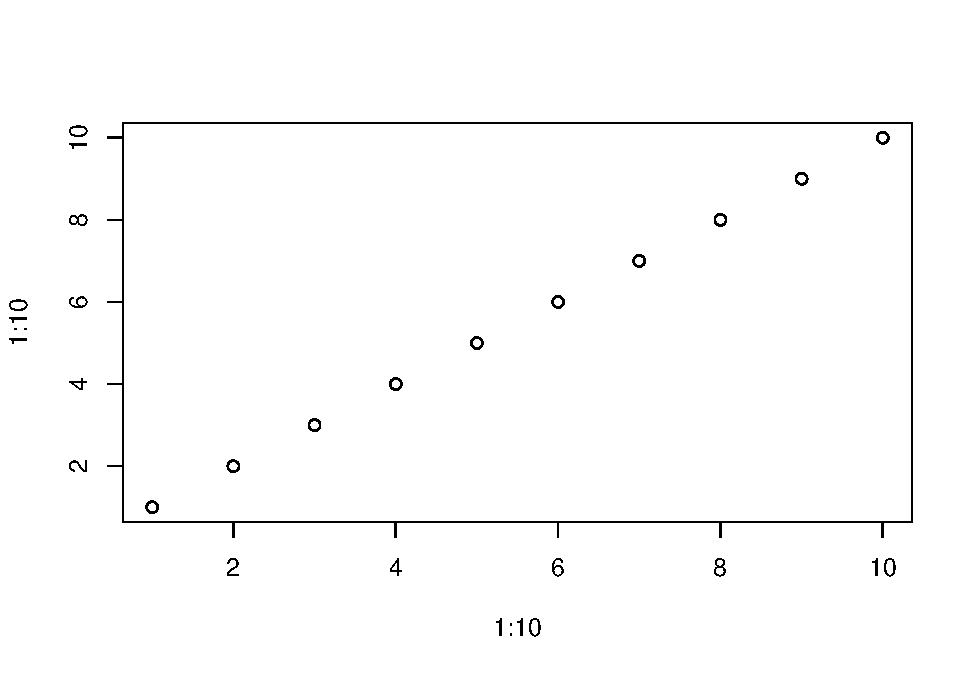
\includegraphics{presencial_função_plot_04_turma_B_files/figure-latex/unnamed-chunk-1-1.pdf}

\begin{Shaded}
\begin{Highlighting}[]
\CommentTok{\# equivalente a:}

\FunctionTok{plot}\NormalTok{( }\DecValTok{1}\SpecialCharTok{:}\DecValTok{10}\NormalTok{ )}
\end{Highlighting}
\end{Shaded}

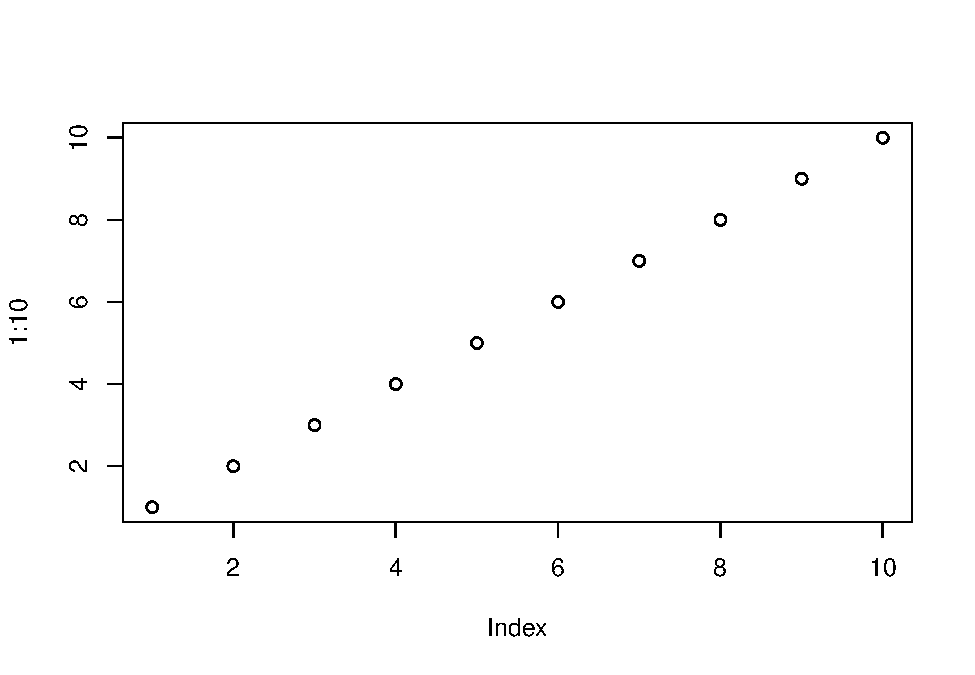
\includegraphics{presencial_função_plot_04_turma_B_files/figure-latex/unnamed-chunk-1-2.pdf}

\hypertarget{alterando-tipos-de-gruxe1fico}{%
\subsubsection{Alterando tipos de
gráfico}\label{alterando-tipos-de-gruxe1fico}}

\hypertarget{gruxe1fico-de-linhas---l}{%
\paragraph{1. gráfico de linhas -
``l''}\label{gruxe1fico-de-linhas---l}}

\begin{Shaded}
\begin{Highlighting}[]
\FunctionTok{plot}\NormalTok{( }\DecValTok{1}\SpecialCharTok{:}\DecValTok{10}\NormalTok{, }\AttributeTok{type =} \StringTok{"l"}\NormalTok{ )}
\end{Highlighting}
\end{Shaded}

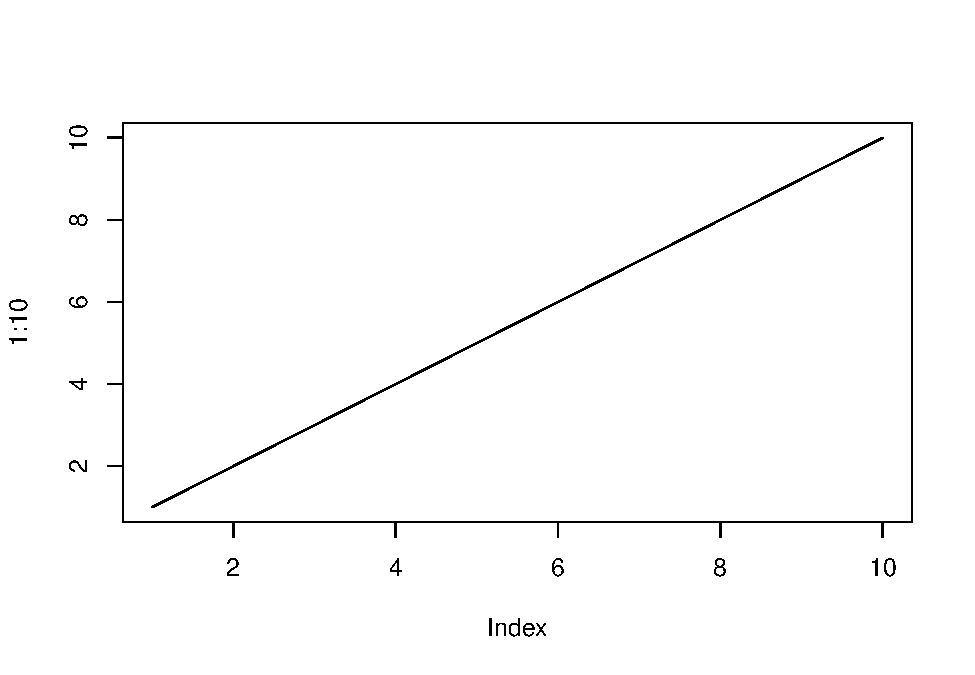
\includegraphics{presencial_função_plot_04_turma_B_files/figure-latex/unnamed-chunk-2-1.pdf}

\hypertarget{gruxe1fico-de-pontos-com-linhas---b}{%
\paragraph{2. gráfico de pontos com linhas -
``b''}\label{gruxe1fico-de-pontos-com-linhas---b}}

\begin{Shaded}
\begin{Highlighting}[]
\FunctionTok{plot}\NormalTok{( }\DecValTok{1}\SpecialCharTok{:}\DecValTok{10}\NormalTok{, }\AttributeTok{type =} \StringTok{"b"}\NormalTok{ )}
\end{Highlighting}
\end{Shaded}

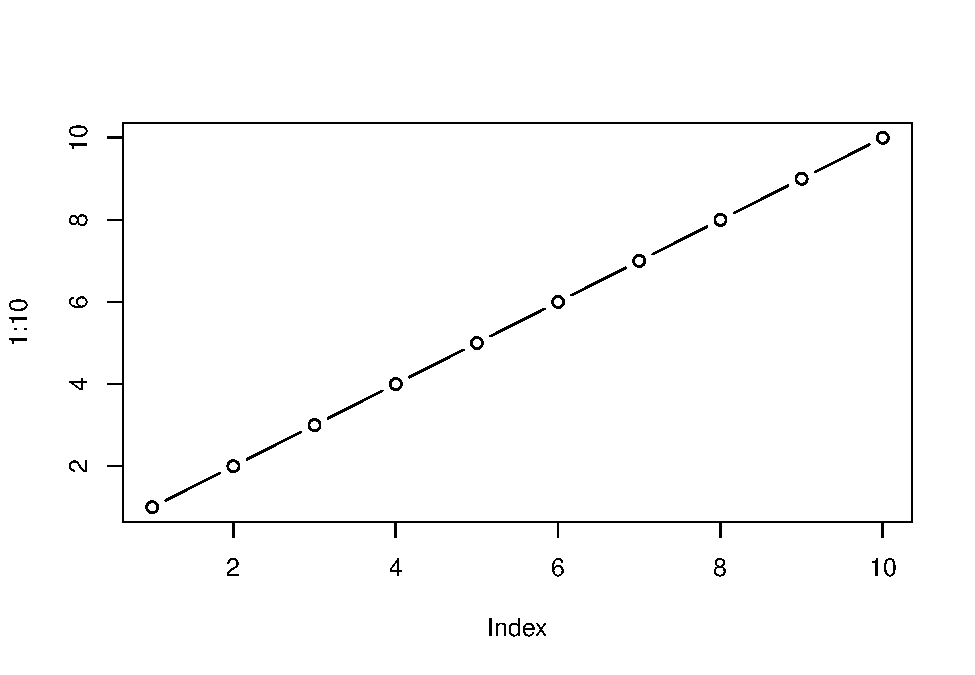
\includegraphics{presencial_função_plot_04_turma_B_files/figure-latex/unnamed-chunk-3-1.pdf}

\hypertarget{gruxe1fico-de-linhas-com-pausas---c}{%
\paragraph{3. gráfico de linhas com ``pausas'' -
``c''}\label{gruxe1fico-de-linhas-com-pausas---c}}

\begin{Shaded}
\begin{Highlighting}[]
\FunctionTok{plot}\NormalTok{( }\DecValTok{1}\SpecialCharTok{:}\DecValTok{10}\NormalTok{, }\AttributeTok{type =} \StringTok{"c"}\NormalTok{ )}
\end{Highlighting}
\end{Shaded}

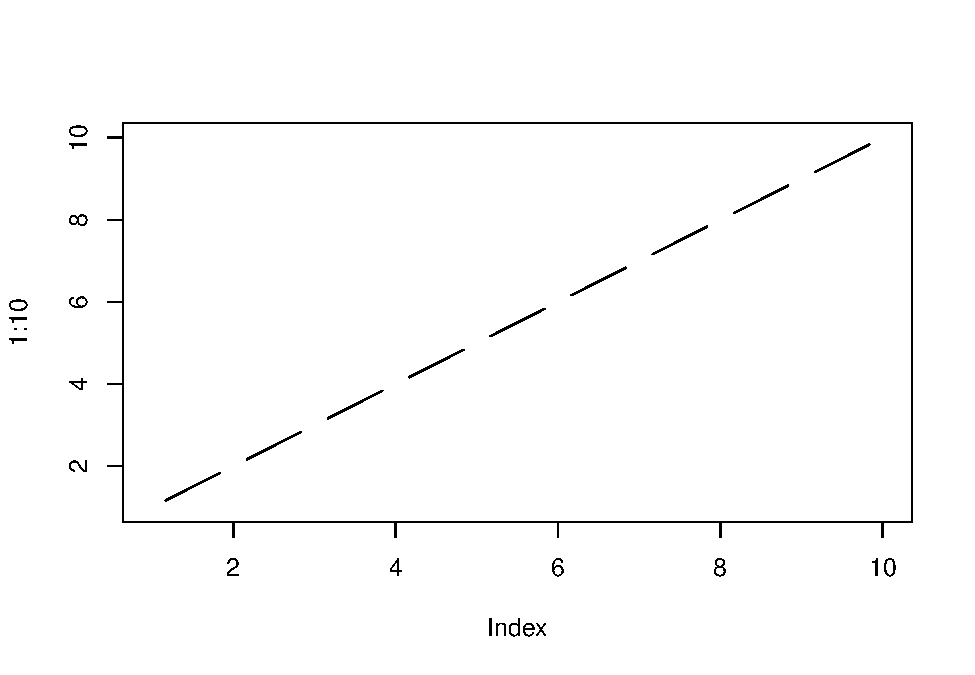
\includegraphics{presencial_função_plot_04_turma_B_files/figure-latex/unnamed-chunk-4-1.pdf}

\hypertarget{gruxe1fico-de-pontos-com-linhas-passando-dentro-dos-pontos---o}{%
\paragraph{4. gráfico de pontos com linhas passando dentro dos pontos -
``o''}\label{gruxe1fico-de-pontos-com-linhas-passando-dentro-dos-pontos---o}}

\begin{Shaded}
\begin{Highlighting}[]
\FunctionTok{plot}\NormalTok{( }\DecValTok{1}\SpecialCharTok{:}\DecValTok{10}\NormalTok{, }\AttributeTok{type =} \StringTok{"o"}\NormalTok{ )}
\end{Highlighting}
\end{Shaded}

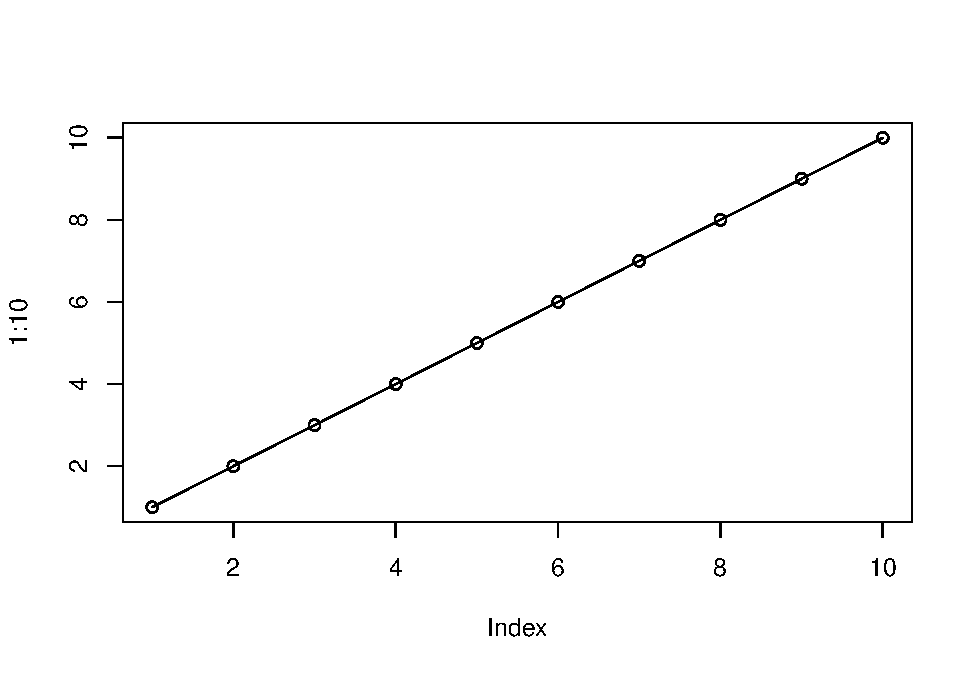
\includegraphics{presencial_função_plot_04_turma_B_files/figure-latex/unnamed-chunk-5-1.pdf}

\hypertarget{gruxe1fico-de-linhas-verticais---h}{%
\paragraph{5. gráfico de linhas verticais -
``h''}\label{gruxe1fico-de-linhas-verticais---h}}

\begin{Shaded}
\begin{Highlighting}[]
\FunctionTok{plot}\NormalTok{( }\DecValTok{1}\SpecialCharTok{:}\DecValTok{10}\NormalTok{, }\AttributeTok{type =} \StringTok{"h"}\NormalTok{ )}
\end{Highlighting}
\end{Shaded}

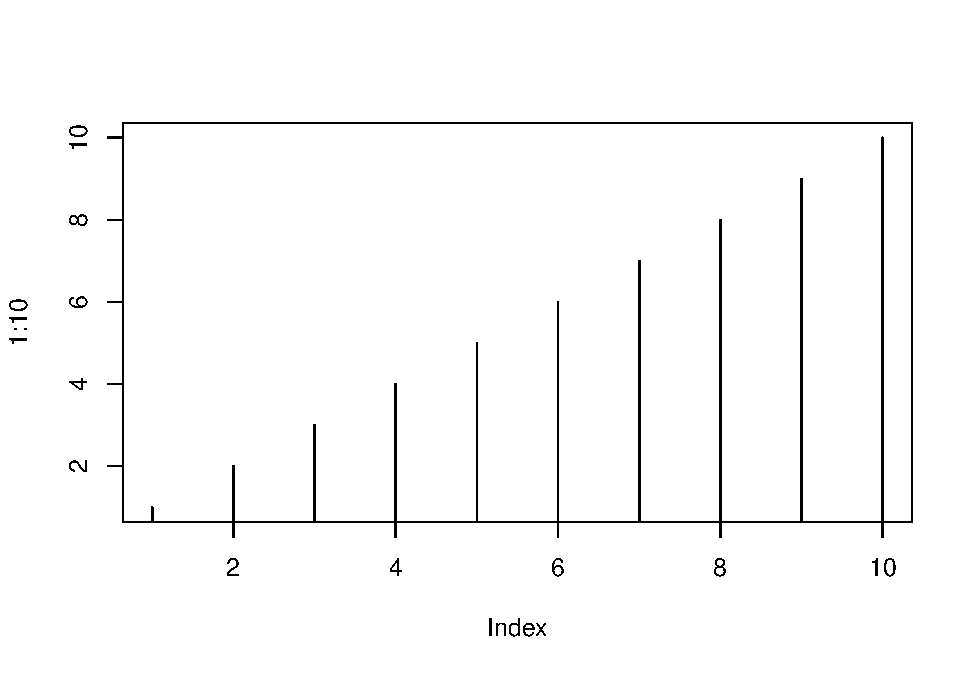
\includegraphics{presencial_função_plot_04_turma_B_files/figure-latex/unnamed-chunk-6-1.pdf}

\hypertarget{gruxe1fico-de-escada---s}{%
\paragraph{6. gráfico de escada -
``s''}\label{gruxe1fico-de-escada---s}}

\begin{Shaded}
\begin{Highlighting}[]
\FunctionTok{plot}\NormalTok{( }\DecValTok{1}\SpecialCharTok{:}\DecValTok{10}\NormalTok{, }\AttributeTok{type =} \StringTok{"s"}\NormalTok{ )}
\end{Highlighting}
\end{Shaded}

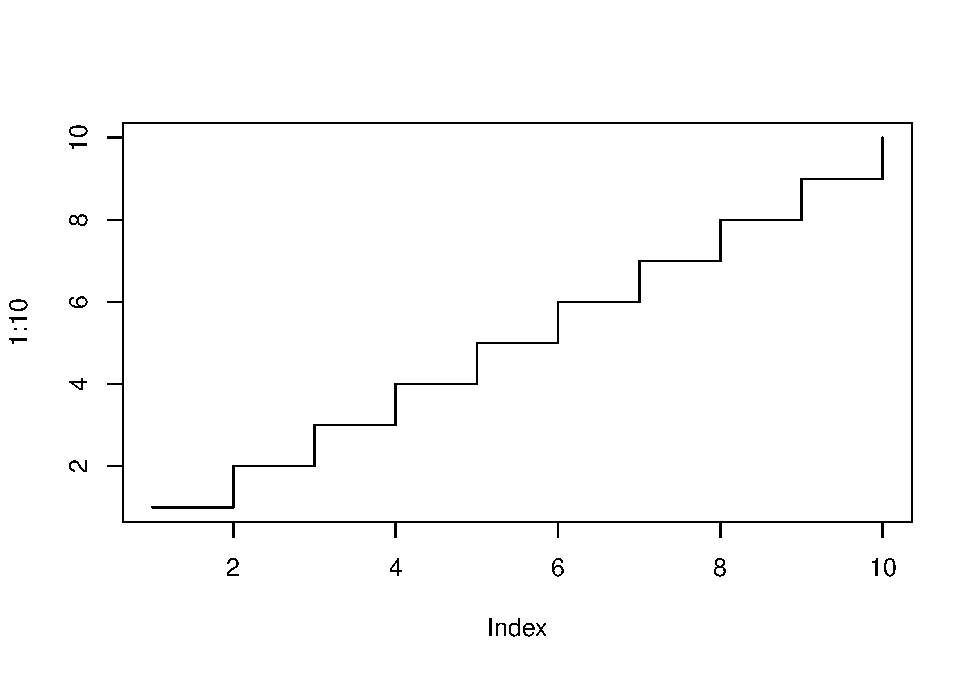
\includegraphics{presencial_função_plot_04_turma_B_files/figure-latex/unnamed-chunk-7-1.pdf}

\hypertarget{gruxe1fico-sem-nada}{%
\paragraph{7. gráfico sem nada}\label{gruxe1fico-sem-nada}}

\begin{Shaded}
\begin{Highlighting}[]
\FunctionTok{plot}\NormalTok{( }\DecValTok{1}\SpecialCharTok{:}\DecValTok{10}\NormalTok{, }\AttributeTok{type =} \StringTok{"n"}\NormalTok{ )}
\end{Highlighting}
\end{Shaded}

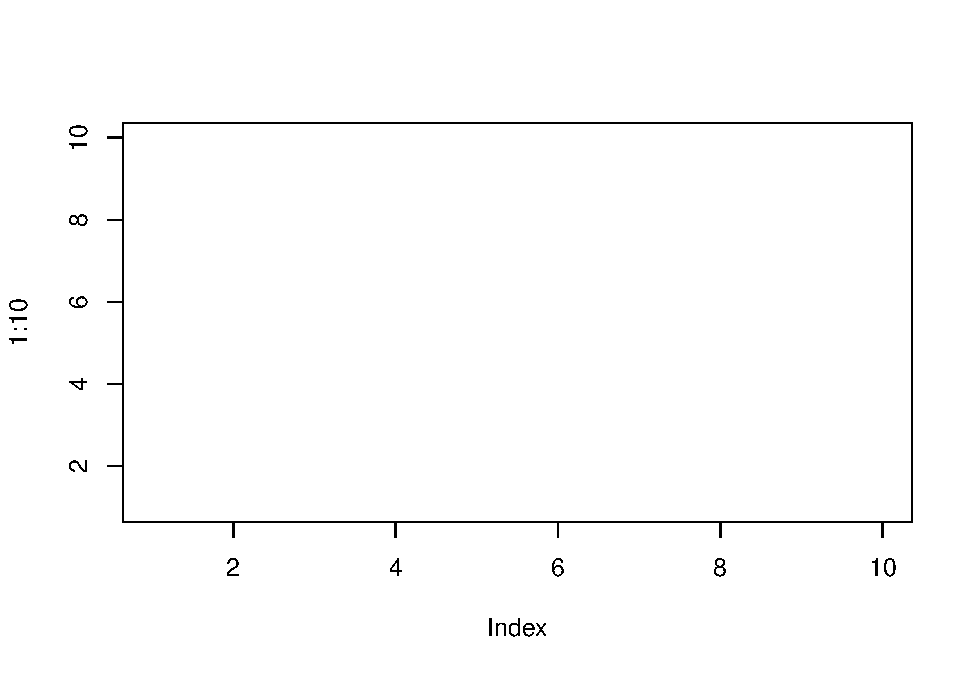
\includegraphics{presencial_função_plot_04_turma_B_files/figure-latex/unnamed-chunk-8-1.pdf}

\hypertarget{alterando-tipos-de-linhas-dos-gruxe1ficos}{%
\subsubsection{Alterando tipos de linhas dos
gráficos}\label{alterando-tipos-de-linhas-dos-gruxe1ficos}}

\hypertarget{para-nuxe3o-termos-que-ocupar-tanto-espauxe7o-como-anteriormente-utilizaremos-um-loop}{%
\paragraph{Para não termos que ocupar tanto espaço como anteriormente,
utilizaremos um
loop}\label{para-nuxe3o-termos-que-ocupar-tanto-espauxe7o-como-anteriormente-utilizaremos-um-loop}}

\hypertarget{para-ver-as-opuxe7uxf5es-de-linhas-disponuxedveis}{%
\paragraph{para ver as opções de linhas
disponíveis}\label{para-ver-as-opuxe7uxf5es-de-linhas-disponuxedveis}}

\begin{Shaded}
\begin{Highlighting}[]
\FunctionTok{par}\NormalTok{( }\AttributeTok{mfrow =} \FunctionTok{c}\NormalTok{( }\DecValTok{2}\NormalTok{, }\DecValTok{3}\NormalTok{ ) )}

\ControlFlowTok{for}\NormalTok{( grossura }\ControlFlowTok{in} \DecValTok{1}\SpecialCharTok{:}\DecValTok{10}\NormalTok{ ) }\FunctionTok{plot}\NormalTok{( }\DecValTok{1}\SpecialCharTok{:}\DecValTok{10}\NormalTok{, }\AttributeTok{type =} \StringTok{"l"}\NormalTok{, }\AttributeTok{lty =}\NormalTok{ grossura )}
\end{Highlighting}
\end{Shaded}

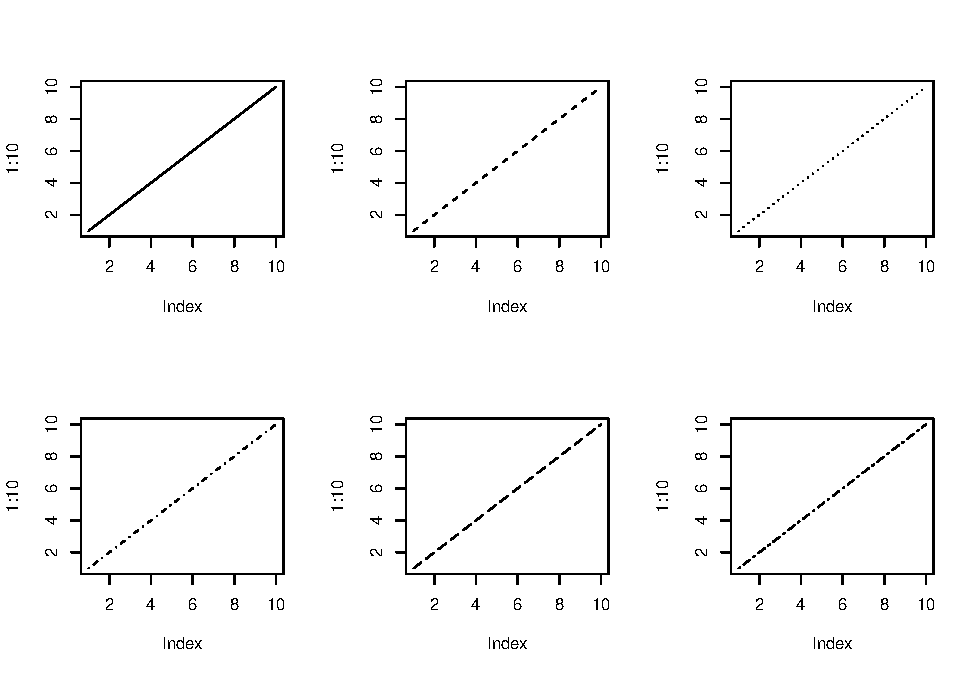
\includegraphics{presencial_função_plot_04_turma_B_files/figure-latex/unnamed-chunk-9-1.pdf}
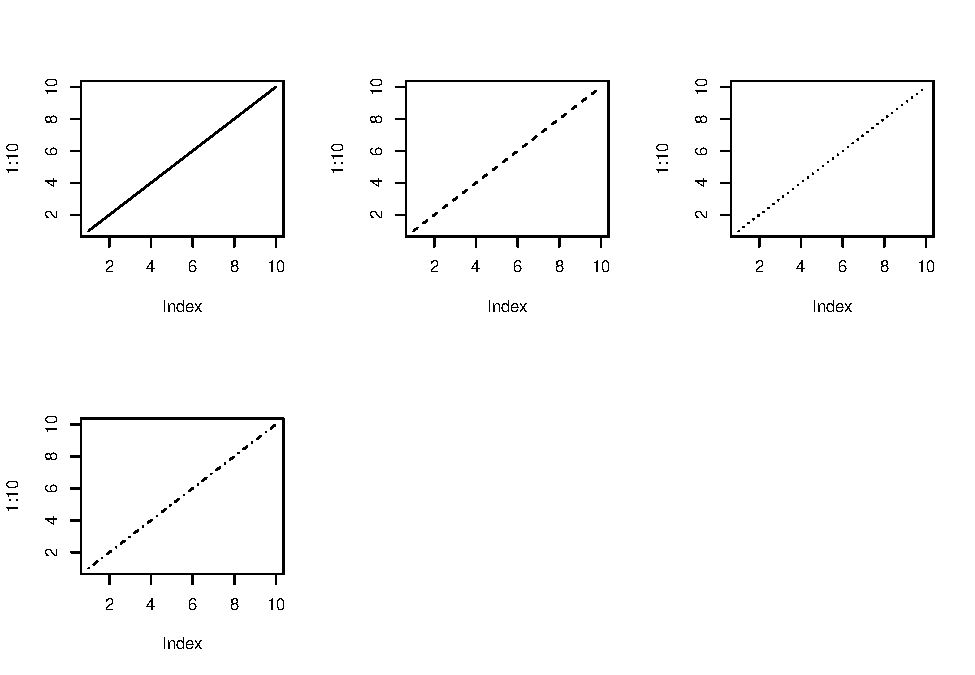
\includegraphics{presencial_função_plot_04_turma_B_files/figure-latex/unnamed-chunk-9-2.pdf}

\hypertarget{alterando-tipos-molduras-dos-gruxe1ficos}{%
\subsubsection{Alterando tipos molduras dos
gráficos}\label{alterando-tipos-molduras-dos-gruxe1ficos}}

\hypertarget{utilizaremos-a-mesma-luxf3gica-mas-dessa-vez-criando-uma-variuxe1vel}{%
\paragraph{Utilizaremos a mesma lógica, mas dessa vez criando uma
variável}\label{utilizaremos-a-mesma-luxf3gica-mas-dessa-vez-criando-uma-variuxe1vel}}

\hypertarget{para-vermos-os-tipos-de-moldura-disponuxedveis-as-quais-podem-ser-encontradas}{%
\paragraph{para vermos os tipos de moldura disponíveis, as quais podem
ser
encontradas}\label{para-vermos-os-tipos-de-moldura-disponuxedveis-as-quais-podem-ser-encontradas}}

\hypertarget{atravuxe9s-do-comando-help-par}{%
\paragraph{\texorpdfstring{através do comando help:
\texttt{?par}}{através do comando help: ?par}}\label{atravuxe9s-do-comando-help-par}}

\begin{Shaded}
\begin{Highlighting}[]
\FunctionTok{par}\NormalTok{( }\AttributeTok{mfrow =} \FunctionTok{c}\NormalTok{( }\DecValTok{2}\NormalTok{, }\DecValTok{2}\NormalTok{ ) )}

\NormalTok{tipos\_graficos }\OtherTok{\textless{}{-}} \FunctionTok{c}\NormalTok{( }\StringTok{"l"}\NormalTok{, }\StringTok{"b"}\NormalTok{, }\StringTok{"c"}\NormalTok{, }\StringTok{"h"}\NormalTok{ ) }

\ControlFlowTok{for}\NormalTok{( tipos }\ControlFlowTok{in}\NormalTok{ tipos\_graficos ) }\FunctionTok{plot}\NormalTok{( }\DecValTok{1}\SpecialCharTok{:}\DecValTok{10}\NormalTok{, }\AttributeTok{type =}\NormalTok{ tipos )}
\end{Highlighting}
\end{Shaded}

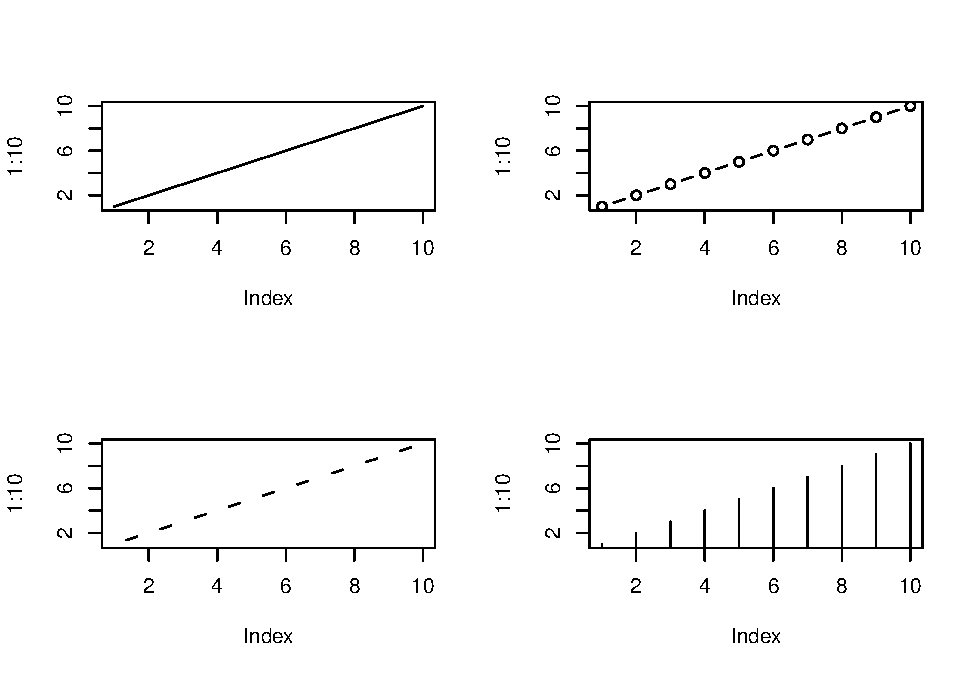
\includegraphics{presencial_função_plot_04_turma_B_files/figure-latex/unnamed-chunk-10-1.pdf}

\hypertarget{alterando-largura-das-linhas-dos-gruxe1ficos}{%
\subsubsection{Alterando largura das linhas dos
gráficos}\label{alterando-largura-das-linhas-dos-gruxe1ficos}}

\begin{Shaded}
\begin{Highlighting}[]
\FunctionTok{par}\NormalTok{( }\AttributeTok{mfrow =} \FunctionTok{c}\NormalTok{( }\DecValTok{2}\NormalTok{, }\DecValTok{5}\NormalTok{ ) )}

\ControlFlowTok{for}\NormalTok{( largura }\ControlFlowTok{in} \DecValTok{1}\SpecialCharTok{:}\DecValTok{10}\NormalTok{ ) }\FunctionTok{plot}\NormalTok{( }\DecValTok{1}\SpecialCharTok{:}\DecValTok{10}\NormalTok{, }\AttributeTok{type =} \StringTok{"l"}\NormalTok{, }\AttributeTok{lwd =}\NormalTok{ largura )}
\end{Highlighting}
\end{Shaded}

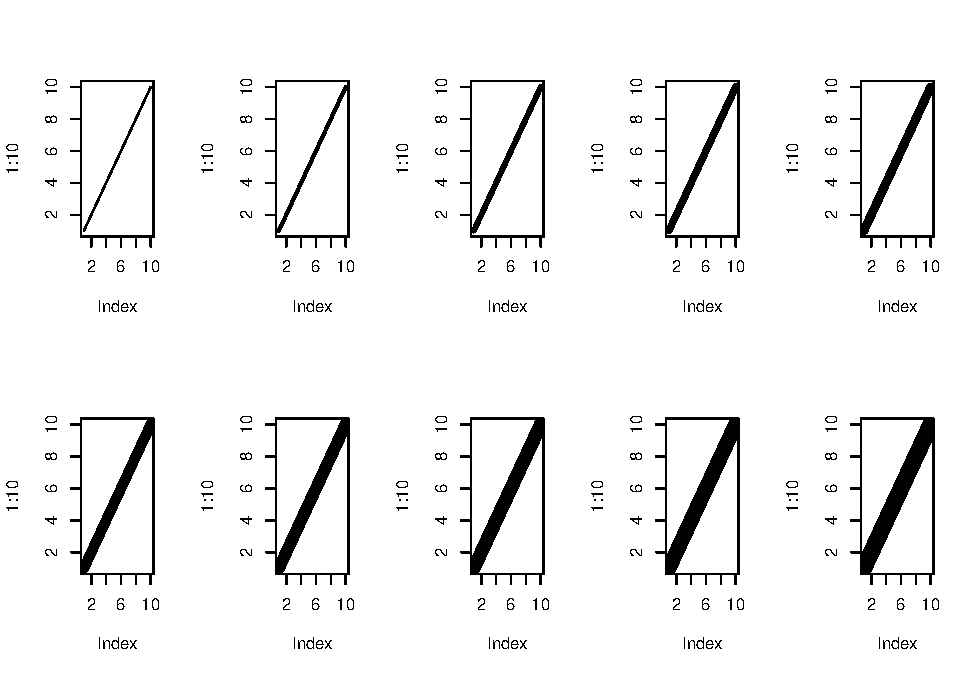
\includegraphics{presencial_função_plot_04_turma_B_files/figure-latex/unnamed-chunk-11-1.pdf}

\hypertarget{alterando-nomes-e-componentes-gruxe1ficos}{%
\subsubsection{Alterando nomes e componentes
gráficos}\label{alterando-nomes-e-componentes-gruxe1ficos}}

\begin{Shaded}
\begin{Highlighting}[]
\FunctionTok{par}\NormalTok{( }\AttributeTok{mfrow =} \FunctionTok{c}\NormalTok{( }\DecValTok{1}\NormalTok{, }\DecValTok{1}\NormalTok{ ) )}

\FunctionTok{plot}\NormalTok{( }\DecValTok{1}\SpecialCharTok{:}\DecValTok{20}\NormalTok{, }\AttributeTok{pch =} \DecValTok{1}\SpecialCharTok{:}\DecValTok{20}\NormalTok{ )}
\end{Highlighting}
\end{Shaded}

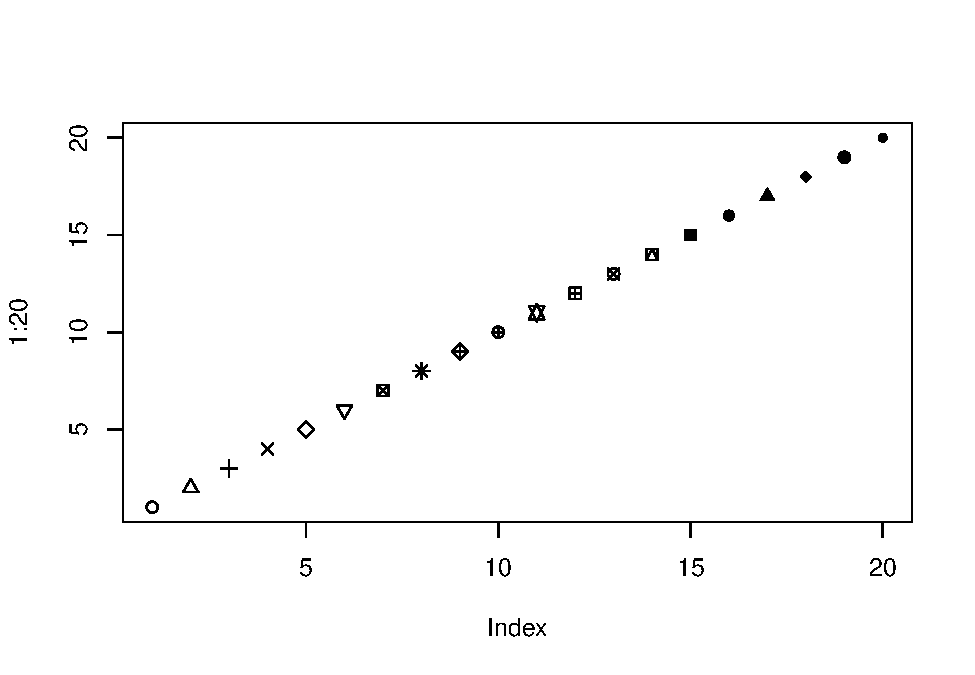
\includegraphics{presencial_função_plot_04_turma_B_files/figure-latex/unnamed-chunk-12-1.pdf}

\begin{Shaded}
\begin{Highlighting}[]
\FunctionTok{plot}\NormalTok{( }\DecValTok{1}\SpecialCharTok{:}\DecValTok{10}\NormalTok{, }\AttributeTok{pch =} \StringTok{"β"}\NormalTok{ )}
\end{Highlighting}
\end{Shaded}

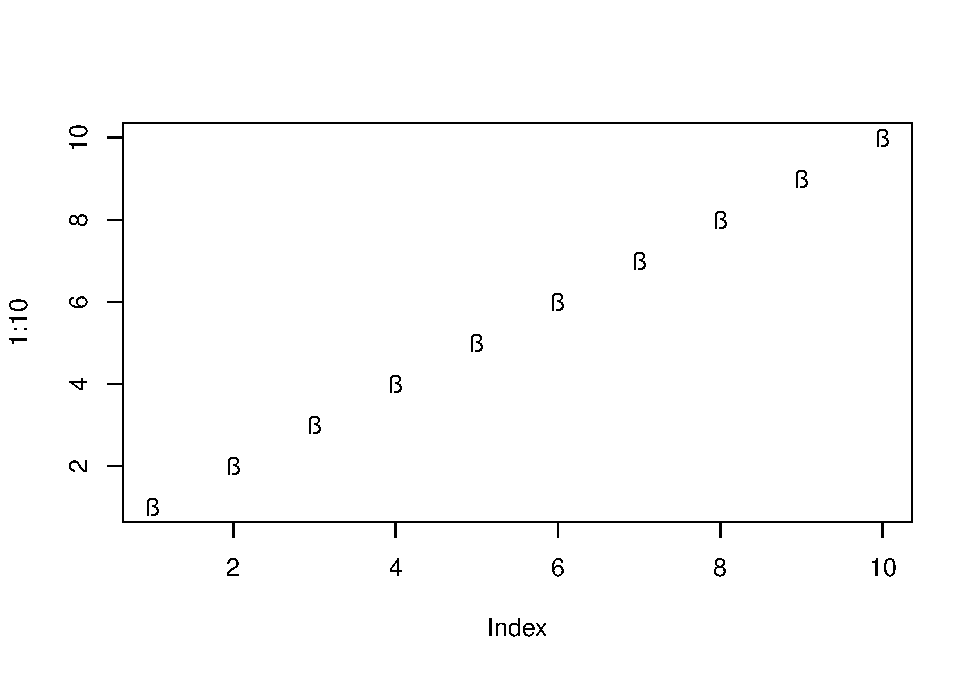
\includegraphics{presencial_função_plot_04_turma_B_files/figure-latex/unnamed-chunk-12-2.pdf}

\begin{Shaded}
\begin{Highlighting}[]
\FunctionTok{plot}\NormalTok{( }\DecValTok{1}\SpecialCharTok{:}\DecValTok{10}\NormalTok{, }\AttributeTok{xlab =} \StringTok{"Eixo x"}\NormalTok{, }\AttributeTok{ylab =} \StringTok{"Eixo y"}\NormalTok{, }\AttributeTok{pch =} \StringTok{"ξ"}\NormalTok{, }\AttributeTok{main =} \StringTok{"Título"}\NormalTok{ )}
\end{Highlighting}
\end{Shaded}

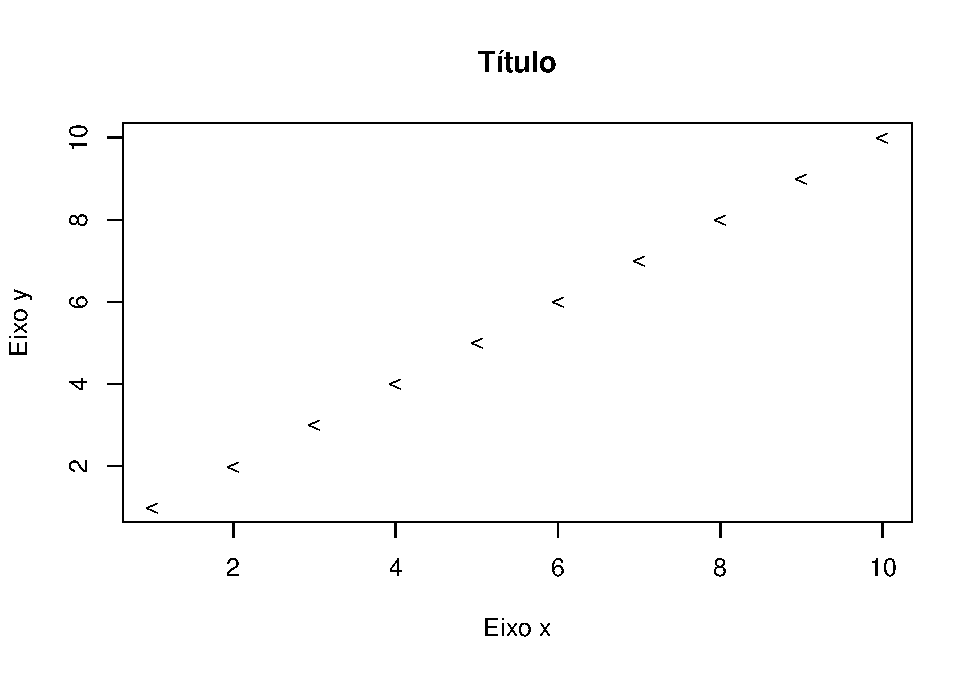
\includegraphics{presencial_função_plot_04_turma_B_files/figure-latex/unnamed-chunk-12-3.pdf}

\hypertarget{exemplo-usando-conjunto-de-dados-do-r}{%
\section{Exemplo usando conjunto de dados do
R}\label{exemplo-usando-conjunto-de-dados-do-r}}

\hypertarget{uxe1rvores-de-cerejeiras-negras}{%
\paragraph{Árvores de cerejeiras
negras}\label{uxe1rvores-de-cerejeiras-negras}}

\begin{Shaded}
\begin{Highlighting}[]
\FunctionTok{data}\NormalTok{()}
\NormalTok{trees}
\end{Highlighting}
\end{Shaded}

\begin{verbatim}
##    Girth Height Volume
## 1    8.3     70   10.3
## 2    8.6     65   10.3
## 3    8.8     63   10.2
## 4   10.5     72   16.4
## 5   10.7     81   18.8
## 6   10.8     83   19.7
## 7   11.0     66   15.6
## 8   11.0     75   18.2
## 9   11.1     80   22.6
## 10  11.2     75   19.9
## 11  11.3     79   24.2
## 12  11.4     76   21.0
## 13  11.4     76   21.4
## 14  11.7     69   21.3
## 15  12.0     75   19.1
## 16  12.9     74   22.2
## 17  12.9     85   33.8
## 18  13.3     86   27.4
## 19  13.7     71   25.7
## 20  13.8     64   24.9
## 21  14.0     78   34.5
## 22  14.2     80   31.7
## 23  14.5     74   36.3
## 24  16.0     72   38.3
## 25  16.3     77   42.6
## 26  17.3     81   55.4
## 27  17.5     82   55.7
## 28  17.9     80   58.3
## 29  18.0     80   51.5
## 30  18.0     80   51.0
## 31  20.6     87   77.0
\end{verbatim}

\hypertarget{personalizando-gruxe1fico-de-circunferuxeancia-por-altura-usando-conceitos-estudados-nesse-encontro-e-no-anterior}{%
\paragraph{Personalizando gráfico de Circunferência por Altura usando
conceitos estudados nesse encontro e no
anterior}\label{personalizando-gruxe1fico-de-circunferuxeancia-por-altura-usando-conceitos-estudados-nesse-encontro-e-no-anterior}}

\begin{Shaded}
\begin{Highlighting}[]
\FunctionTok{plot}\NormalTok{( }\AttributeTok{x =}\NormalTok{ trees}\SpecialCharTok{$}\NormalTok{Height, }\AttributeTok{y =}\NormalTok{ trees}\SpecialCharTok{$}\NormalTok{Girth,}
      \AttributeTok{xlab =} \StringTok{"Altura"}\NormalTok{, }\AttributeTok{ylab =} \StringTok{"Circunferência"}\NormalTok{, }\AttributeTok{main =} \StringTok{"Cerejeira Negra"}\NormalTok{,}
      \AttributeTok{pch =} \DecValTok{7}\NormalTok{ )}
\end{Highlighting}
\end{Shaded}

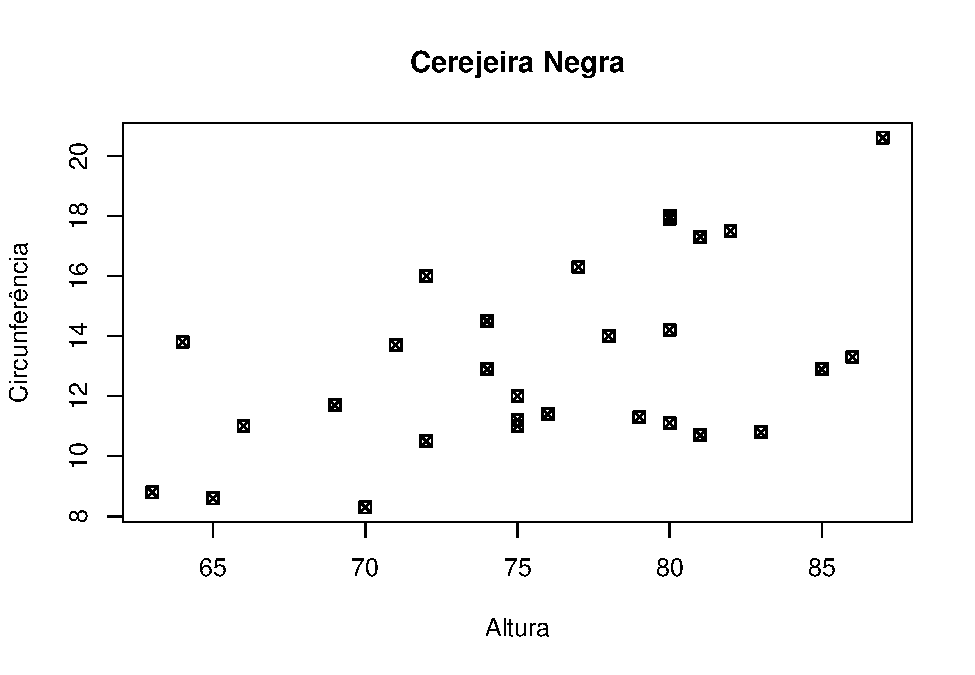
\includegraphics{presencial_função_plot_04_turma_B_files/figure-latex/unnamed-chunk-14-1.pdf}

\hypertarget{histograma}{%
\paragraph{Histograma}\label{histograma}}

\begin{Shaded}
\begin{Highlighting}[]
\FunctionTok{hist}\NormalTok{( trees}\SpecialCharTok{$}\NormalTok{Height, }\AttributeTok{freq =} \ConstantTok{TRUE}\NormalTok{, }\AttributeTok{col =} \FunctionTok{terrain.colors}\NormalTok{( }\DecValTok{10}\NormalTok{ ), }\AttributeTok{ylab =} \StringTok{"Altura"}\NormalTok{,}
      \AttributeTok{xlab =} \StringTok{"Frequência"}\NormalTok{, }\AttributeTok{main =} \StringTok{"Histograma"}\NormalTok{ )}

\FunctionTok{legend}\NormalTok{( }\AttributeTok{x =} \StringTok{"topright"}\NormalTok{, }\AttributeTok{legen =} \StringTok{"Altura"}\NormalTok{, }\AttributeTok{col =} \StringTok{"green"}\NormalTok{ )}
\end{Highlighting}
\end{Shaded}

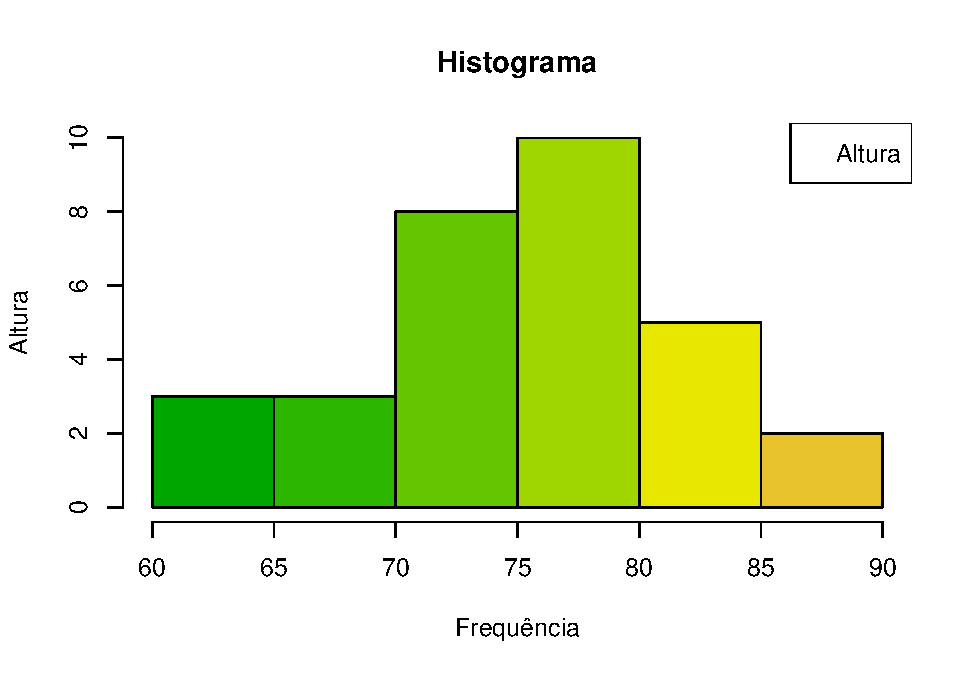
\includegraphics{presencial_função_plot_04_turma_B_files/figure-latex/unnamed-chunk-15-1.pdf}

\begin{Shaded}
\begin{Highlighting}[]
\CommentTok{\# criando a linha da regressão linear: }
\end{Highlighting}
\end{Shaded}


\end{document}
